%%%%%%%%%%%%%%%%%%%%%%%%%%%%%%%%%%%%%%%%%
% Tufte Essay
% LaTeX Template
% Version 2.0 (19/1/19)
%
% This template originates from:
% http://www.LaTeXTemplates.com
%
% Authors:
% The Tufte-LaTeX Developers (https://www.ctan.org/pkg/tufte-latex)
% Vel (vel@LaTeXTemplates.com)
%
% License:
% Apache License, version 2.0
%
%%%%%%%%%%%%%%%%%%%%%%%%%%%%%%%%%%%%%%%%%

%----------------------------------------------------------------------------------------
%	PACKAGES AND OTHER DOCUMENT CONFIGURATIONS
%----------------------------------------------------------------------------------------

\documentclass[a4paper]{tufte-handout} % Use A4 paper by default, remove 'a4paper' for US letter

\usepackage{graphicx} % Required for including images
\setkeys{Gin}{width=\linewidth, totalheight=\textheight, keepaspectratio} % Default images settings
\graphicspath{{Figures/}{./}} % Specifies where to look for included images (trailing slash required)

\usepackage{amsmath, amsfonts, amssymb, amsthm} % For math equations, theorems, symbols, etc
\usepackage{units} % Non-stacked fractions and better unit spacing

\usepackage{booktabs} % Required for better horizontal rules in tables
\usepackage{subfigure}
\usepackage{parskip}
\usepackage{tikz}
\usetikzlibrary{graphs, positioning, quotes, shapes.geometric}
\usepackage{booktabs}

\usepackage{array, caption, threeparttable}


%----------------------------------------------------------------------------------------
%	TITLE SECTION
%----------------------------------------------------------------------------------------

\title{Audio Program Design and Application - 7}

\author{Chuhan Qiu}


%----------------------------------------------------------------------------------------

\begin{document}

\maketitle % Print the title section

%----------------------------------------------------------------------------------------
%	ABSTRACT/SUMMARY
%----------------------------------------------------------------------------------------

\begin{abstract}
	\textbf{Summary}
In this report, I implement four comb filters, and comparing their performance, including design specification and perception evaluation. Comb filter is actually the basic component of delay effect, so on the basis of them, I apply delay effect to one audio signal and design a subjective evaluation experiment. In addition, among them, the natural comb filter is also called low-pass IIR comb filter, which is added an one-pole low-pass filter in its feedback loop. I extend this and try to add similar structures to different loops of two comb filters, including IIR comb filter and universal comb filter.
\end{abstract}

%----------------------------------------------------------------------------------------
%	ESSAY BODY
%----------------------------------------------------------------------------------------

\section{INTRODUCTION}
Comb filter can be used to implement the delay effect in many ways, which also brings different sound effects. Generally, the comb filters can be divided into IIR structure and FIR structure, whose main difference is shown in Figure 1.

\begin{figure}[h!]
    \centering
    \subfigure[FIR Comb Filter]{
        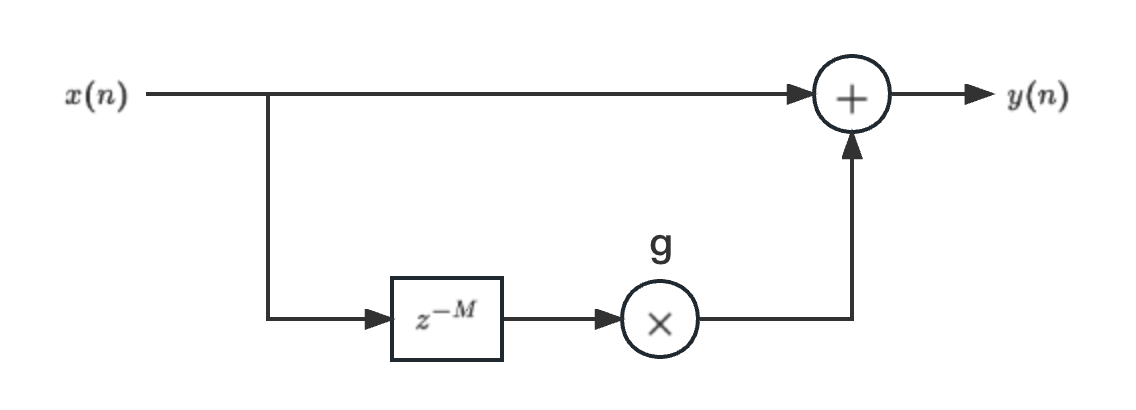
\includegraphics[width=3in]{Image/FIRComb.png}
    }
    \subfigure[IIR Comb Filter]{
	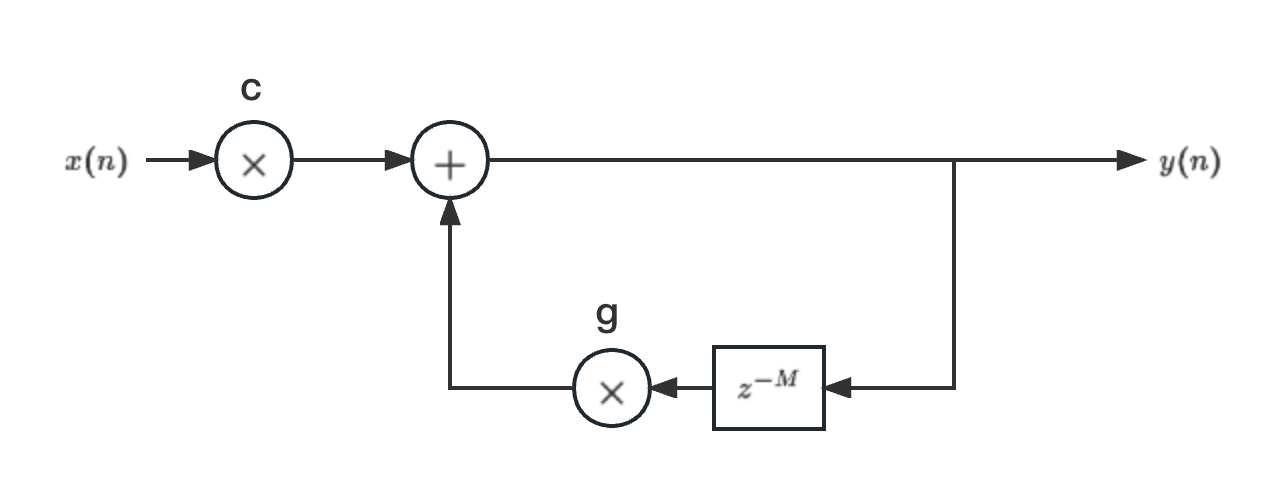
\includegraphics[width=3in]{Image/IIRComb.png}
    }
    \caption{Different Structures Comb Filter Comparison}
\end{figure}

Obviously, IIR comb filter contains a feedback loop, which is the main difference between it and FIR comb filter. Besides, DAFX\footnote{Udo Zölzer, 2011, DAFX: Digital Audio Effects, /10.1002/9781119991298} introduced universal comb filter, by combining the IIR and FIR comb filter which is shown as Figure 2.
\begin{figure}[h]
    \centering
	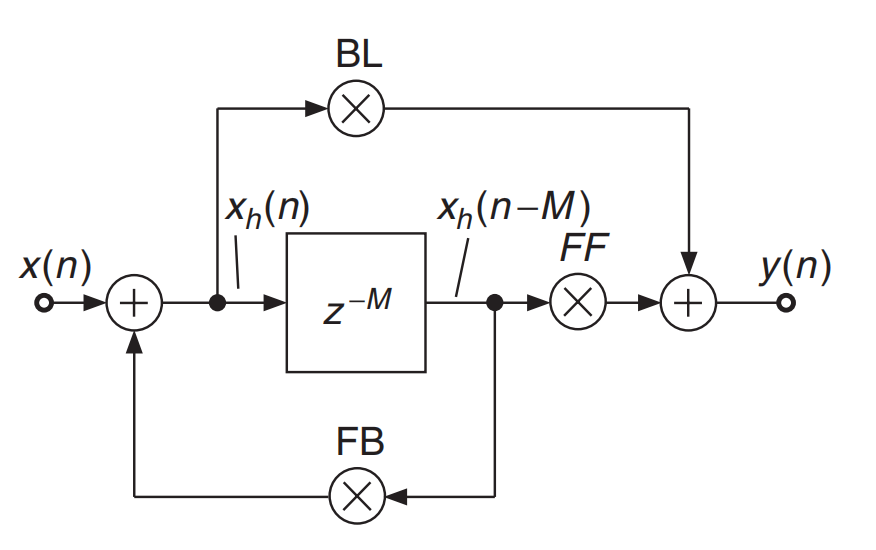
\includegraphics[width=2.5in]{Image/UniversalComb.png}
	\caption{Universial Comb Filter}
	\label{fig:textfig}
	\setfloatalignment{a} % Position the figure caption in the middle of the figure
\end{figure}

The structure shown in Figure 2 can also form all-pass filter and delay effect beside FIR and IIR comb filter by adjusting the value of modules 'BL', 'FB' and 'FF' as shown in table 1. In addition, by introducing parallel connection of $N$ comb filter which is shown in Figure 2, further adjusting the parameter then different effects could be implemented. And this structure is called 'generalized comb filter' in DAFX.

\begin{table}[ht]
	\centering
	\fontfamily{ppl}\selectfont
	\begin{tabular}{l l l l}
		\toprule
		 & BL & FB & FF \\
		\midrule
		FIR comb filter & 1 & 0 & g \\
		IIR comb filter & c & g & 0 \\
		Allpass & a & -a & 1 \\
		Delay   & 0 &  0 & 1 \\
		\bottomrule
	\end{tabular}
	\caption{Parameters for universal comb filter}
	\label{tab:normaltab}
	\setfloatalignment{b} % Position the table caption at the bottom of the table
\end{table}

\begin{figure}[h]
    \centering
	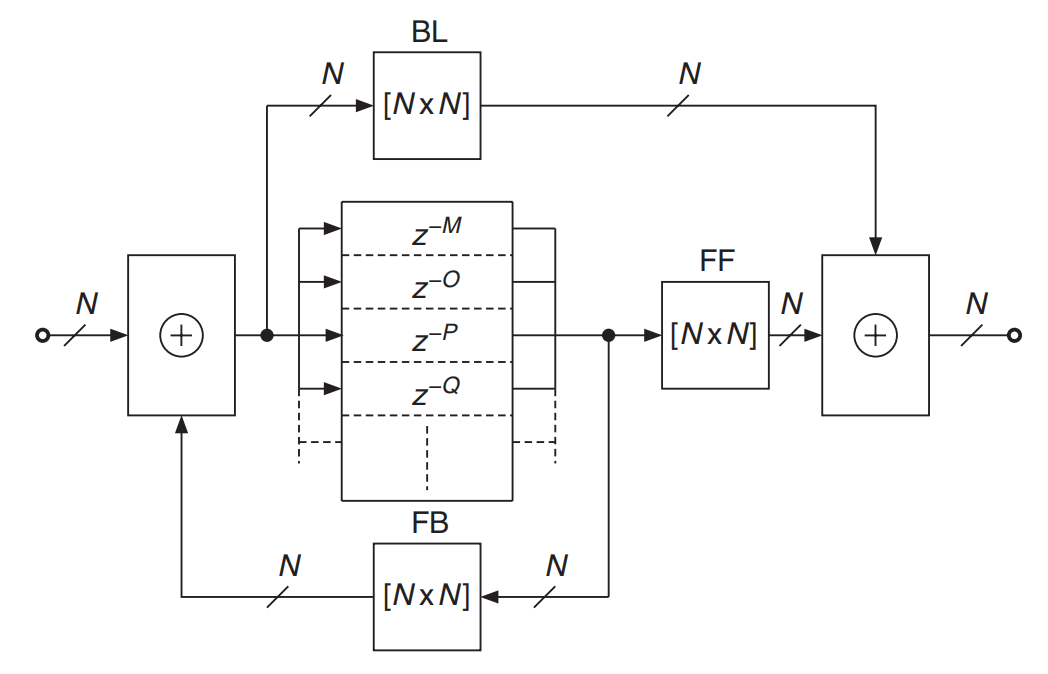
\includegraphics[width=3in]{Image/ParallelComb.png}
	\caption{Generalized structure of parallel allpass comb filters}
	\label{fig:textfig}
	\setfloatalignment{a} % Position the figure caption in the middle of the figure
\end{figure}

\begin{table}[ht]
	\centering
	\fontfamily{ppl}\selectfont
	\begin{tabular}{l l l l l}
		\toprule
		 & Delay & BL & FB & FF \\
		\midrule
		Slapback & 50 ms & 1 & 0 & X \\
		Echo & >50 ms & 1 & 0 < X < 1 & 0 \\
		Reverb &  & Matrix & Matrix & Matrix \\
		\bottomrule
	\end{tabular}
	\caption{Parameters for generalized comb filter}
	\label{tab:normaltab}
	\setfloatalignment{b} % Position the table caption at the bottom of the table
\end{table}

Then, if we replace the normal delay line in universal comb filter by fractional delay line(which also called variable-length delay line in DAFX), we can obtain many industry standard audio effects. The main idea of it is based on the all-pass filter modification towards an universal comb filter, and the structure of it is shown as Figure 4. Wherein $MOD(n)$ is also called 'control signal', actually $MOD(n)$ as a modulator for the delay line leads to the time-varying frequency of whole filter and produces vibrato effect.
\begin{figure}[h]
    \centering
	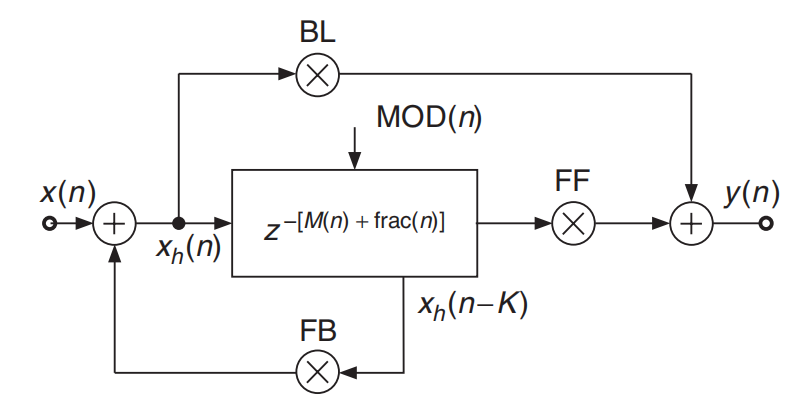
\includegraphics[width=3in]{Image/VariableDelayComb.png}
	\caption{Standard effects with variable-length delay line}
	\label{fig:textfig}
	\setfloatalignment{a} % Position the figure caption in the middle of the figure
\end{figure}

\begin{table}[ht]
    \caption{Industry standard audio effects}
	\centering
	\fontfamily{ppl}\selectfont
	\begin{tabular}{l l l l l l l}
		\toprule
		 & BL & FF & FB & Delay & Depth & MOD \\
		\midrule
		Vibrato & 0 & 1 & 0 & 0 ms & 0–3 ms & 0.1–5 Hz sine \\
		Flanger & 0.7 & 0.7 & 0.7 & 0 ms & 0–2 ms & 0.1–1 Hz sine \\
		(White)Chorus & 0.7 & 1 & -0.7 & 1-30 ms & 1-30 ms & Lowpass noise\\
		Doubling & 0.7 & 0.7 & 0 & 10–100 ms & 1–100 ms & Lowpass noise \\
		\bottomrule
	\end{tabular}
\end{table}

However, parameters 'Depth' and 'MOD' look quite abrupt among them, which are not even reflected in the flow chart. In fact, the fractional delay line is equal to phase modulation. Applying phase modulation to audio signals for audio effects will modify the phase of the audio signal $x(n)$ by a control parameter or modulating signal $m(n)$, which is equivalent to the $MOD(n)$ in generalized structure. To describe the system of a phase modulator, DAFX introduced a time-variant impulse response $h(n)$ and leads to a phase modulated output signal $x_{PM}(n)$. Then phase modulation process is as equation (1) and (2).
\begin{equation}
h(n)=\delta[n-m(n)]
\end{equation}

\begin{equation}
y(n)=x_{PM}(n)=x(N)·h(n)=x(n) \ast \delta[n-m(n)]
\end{equation}

The result for phase modulation of the signal $x(n)$ can then be written as 
\begin{equation}
y(n)=x_{PM}(n)=x(n-m(n))
\end{equation}

where $m(n)$ is a continuous variable, which changes every discrete time instant $n$. Therefore $m(n)$ is decomposed into an integer and a fractional part, which is the same as fractional delay line.
\begin{figure}[h]
    \centering
	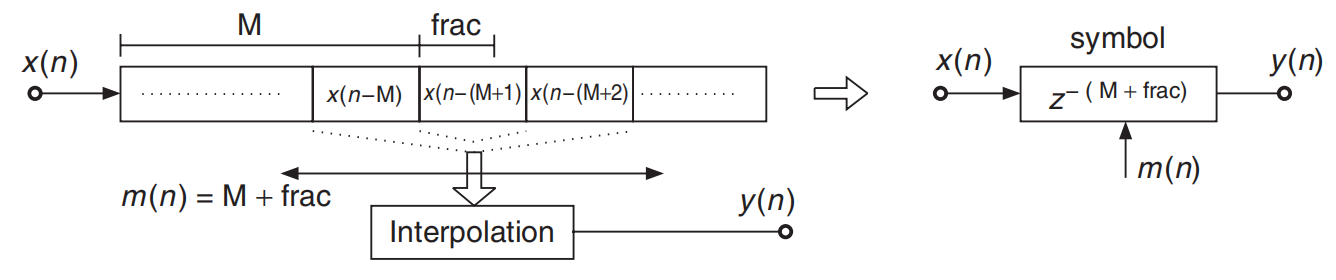
\includegraphics[width=4in]{Image/PhaseModulation.png}
	\caption{Phase modulator based on fractional delay line}
	\label{fig:textfig}
	\setfloatalignment{a} % Position the figure caption in the middle of the figure
\end{figure}

For sine-type modulation, useful for vibrato effects, the modulation signal can be written as
\begin{equation}
m(n)=M+Depth \cdot sin(\omega_MnT)
\end{equation}
That's the meaning of parameter 'Depth' in Table 3.

To simulate the absorption of the high frequencies by the air, Moorer\footnote{J.A. Moorer. About this reverberation business. In Foundations of Computer Music, pp. 605–639.MIT Press, 1985.} introduced a first-order lowpass filter in the feedback loop, which is shown as Figure 6.
\begin{figure}[h]
    \centering
	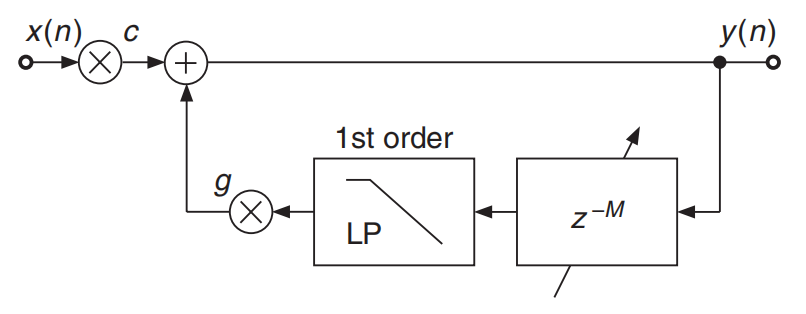
\includegraphics[width=3.5in]{Image/NaturalComb.png}
	\caption{Structure of natural comb filter}
	\label{fig:textfig}
	\setfloatalignment{a} % Position the figure caption in the middle of the figure
\end{figure}

This method makes sound more natural by attenuating high-frequency components of the feedback loop. What's more, similar process can also be used in different loops or even different structures of comb filters to generate new sound effect. In next section, I describe the method I used to implement different structures of comb filters and compare them in different dimensions. After that, in section 3, a subjective perception experiment is proposed to compare the sound effect of them, with the evaluation dimensions set by myself. In section 4, the results of the subjective experiment is shown and they are discussed in section 5.

\section{METHOD}
I implement four comb filters that mentioned in our course, and call them as the encapsulating function. DAFX has provided transform functions for us to implement FIR and IIR comb filters. For FIR comb filter, its transform function is as equation (5).
\begin{equation}
H(z)=1+gz^{-M}
\end{equation}

And IIR comb filter is as equation (6).
\begin{equation}
H(z)=\frac{c}{1-gz^{-M}}
\end{equation}

DAFX didn't give the transform function of universal comb filter, but in our course, the transform function of it is given by
\begin{equation}
H(z)=\frac{BL+FF \cdot z^{-M}}{1-FB \cdot z^{-M}} = \frac{c+g_1z^{-M}}{1-g_2z^{-M}}
\end{equation}

Based on IIR comb filter, the transform function of natural comb filter can be inferred by
\begin{equation}
H(z)=\frac{c}{1-g \cdot (z^{-M} \cdot H_{LP}(z))}
\end{equation}
wherein $H_{LP}(z)$ is the transform function of low-pass filter, which could be set to first-order or second-order. For first-order, the natural comb filter is shown as equation (9).
\begin{equation}
  H_{LP}(z)=\frac{z^{-M}(b_0+b_1z^{-1})}{1+a_1z^{-1}}
\end{equation}

\begin{equation}
\begin{aligned}
  H(z)&=\frac{c}{1-g \cdot (\frac{z^{-M}(b_0+b_1z^{-1})}{1+a_1z^{-1}})} \\
  &=\frac{c(1+a_1z^{-1})}{1+a_1z^{-1}-g \cdot b_0z^{-M}-g \cdot b_1z^{-(M+1)}}
\end{aligned}
\end{equation}

Equation (10) is inferred according to Figure 6. So we can add the same low-pass filter to different loops and obtain new comb filters. First of all, I add the low-pass filter to FIR comb filter's direct path and side-chain(reflected path) respectively. 
And the transform functions are given by
\begin{itemize}
    \item The transform function of adding low-pass to direct path can be inferred by
    \begin{equation}
    \begin{aligned}
        &y(n)=h_{LP}(n) \ast x(n) + gx(n-M) \\
        &H(z)=H_{LP}(z)+gz^{-M} \\
        &=z^{-M}(\frac{b_0+b_1z^{-1}}{1+a_1z^{-1}}+g) \\
        &=\frac{(b_0+g)z^{-M}+(b_1+ga_1)z^{-(M+1)}}{1+a_1z^{-1}}
    \end{aligned}
    \end{equation}
    and the flow chart is shown as Figure 7.
    
    \begin{figure}[h]
    \centering
	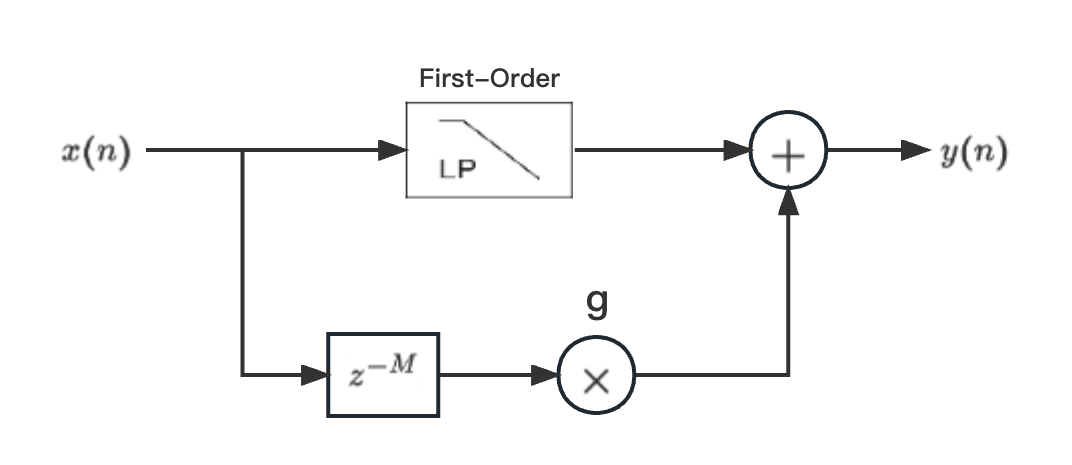
\includegraphics[width=4in]{Image/DirectPath.png}
	\caption{FIR comb filter with low-pass filter in direct path}
	\label{fig:textfig}
	\setfloatalignment{a} % Position the figure caption in the middle of the figure
    \end{figure}
    
    \item Similarly, adding the same low-pass filter to the side-chain of FIR comb filter, and the transform function can be inferred as
    \begin{equation}
    \begin{aligned}
        &y(n)=x(n) + h_{LP} \ast gx(n-M) \\
        &H(z)=1+gz^{-M}H_{LP}(z) \\
        &=1+\frac{gz^{-M}(b_0+b_1z^{-1})}{1+a_1z^{-1}} \\
        &=\frac{1+a_1z^{-1}+b_0gz^{-M}+b_1gz^{-(M+1)}}{1+a_1z^{-1}}
    \end{aligned}
    \end{equation}
    
    
    \begin{figure}[h]
    \centering
	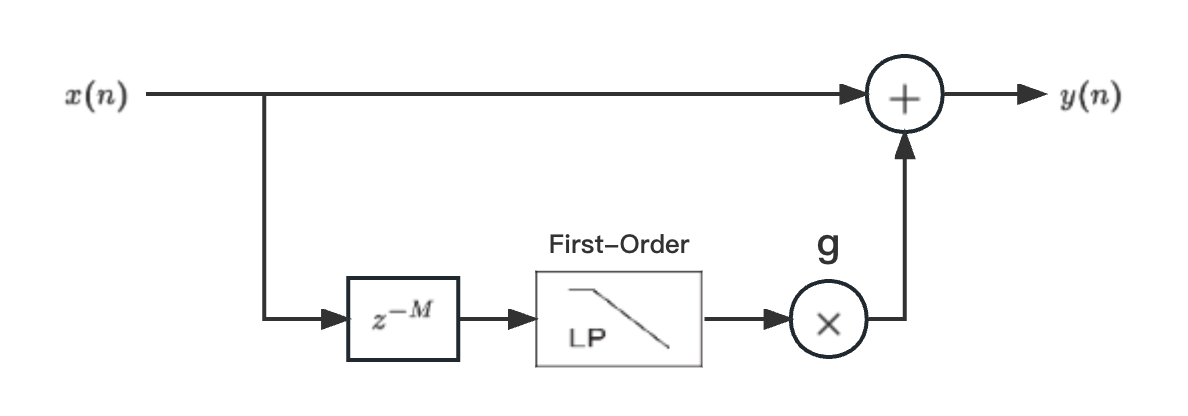
\includegraphics[width=4in]{Image/SideChain.png}
	\caption{FIR comb filter with low-pass filter in side path}
	\label{fig:textfig}
	\setfloatalignment{a} % Position the figure caption in the middle of the figure
    \end{figure}
    
\end{itemize}

Besides, we can also do the same changes to universal comb filter. Here I add low-pass filter to all paths of universal comb filter. The flow chart is shown as Figure 9 and I obtain a new transform function, which can be interred by
\begin{equation}
\begin{cases}
  x_h(n)=x(n)+ FB \cdot x_h(n-M) \ast h_{LP}(n) \ast h_{LP}(n)  \\
  y(n)= BL \cdot x_h(n) \ast h_{LP}(n) + FF \cdot x_h(n-M) \ast h_{LP}(n)
\end{cases}
\end{equation}
Apply Z-transformation on equation (13) and obtain that
\begin{equation}
\begin{cases}
  X_h(z)=X(z) + FB \cdot X_h(z)z^{-M} \cdot H_{LP}(z) \cdot H_{LP}(z)=\frac{X(z)}{1-FB \cdot H_{LP}^2(z)z^{-M}} \\
  Y(z) = BL \cdot X_h(z) \cdot H_{LP}(z) + FF \cdot X_h(z)z^{-M} \cdot H_{LP}(z)
\end{cases}
\end{equation}
Simultaneous equation (14) and obtain that
\begin{equation}
  \begin{aligned}
      &Y(z)=\frac{BL \cdot X(z)}{1-FB \cdot H^2_LP(z)z^{-M}}+\frac{FF \cdot X(z) \cdot H_LP(z)z^{-M}}{1-FB \cdot H^2_{LP}(z)z^{-M}} \\
      &H(z)=\frac{BL+FF \cdot H_{LP}(z)z^{-M}}{1-FB \cdot H_{LP}^2(z)z^{-M}} 
  \end{aligned}
\end{equation}
when $H(z)=\frac{b_0+b_1z^{-1}}{1+a_1z^{-1}}$, equation (15) would be convert to
\begin{equation}
  \begin{aligned}
      H(z)&=\frac{BL+\frac{FF \cdot (b_0+b_1)}{1+a_1z^{-1}}z^{-M}}{1-\frac{FB \cdot (b_0+b_1z^{-1})^2}{(1+a_1z^{-1})^2}z^{-M}} \\
      &=\frac{BL \cdot (1+a_1z^{-1})^2+FF \cdot (b_0+b_1z^{-1})(1+a_1z^{-1})z^{-M}}{(1+a_1z^{-1})^2-FB \cdot (b_0+b_1z^{-1})z^{-M}} \\
      &=\frac{BL+2BLa_1 \cdot z^{-1}+BLa_1^2 \cdot z^{-2}+FF \cdot z^{-M}+FF(b_1+a_1b_0)z^{-(M+1)}+FFa_1b_1 \cdot z^{-(M+2)}}{1+2a_1 \cdot z^{-1}+a_1^2 \cdot z^{-2}-FBb_0^2 \cdot z^{-M}-2FBb_1b_0 \cdot z^{-(M+1)}-FBb_1^2 \cdot z^{-(M+2)}}
  \end{aligned}
\end{equation}

\begin{figure}[h]
    \centering
	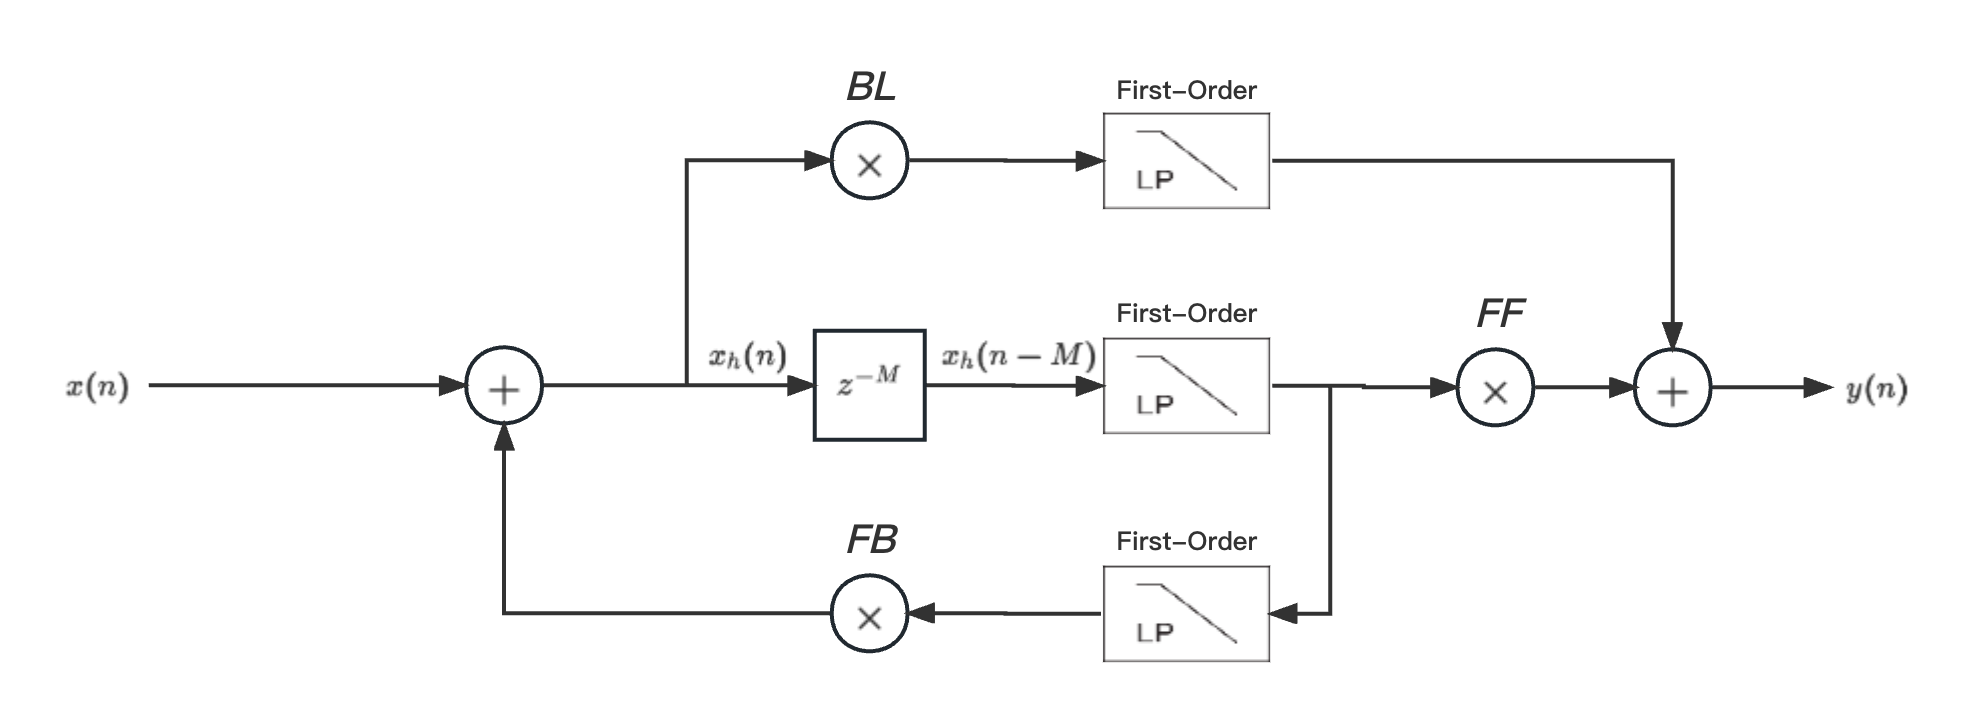
\includegraphics[width=4.5in]{Image/UniversalNatural.png}
	\caption{Natural universal comb filter}
	\label{fig:textfig}
	\setfloatalignment{a} % Position the figure caption in the middle of the figure
\end{figure}

In summary, three new structures and their transform functions have been proposed. Equation (11), (12) and (16) show their numerator and denominator coefficients respectively, which are the keys to implement these filters.

\section{EXPERIMENTAL SETUP}
In this report, I have implemented seven different structure filter in total. To compare the effect that they have brought, I design two separate sets of experiment, one consisting of four types of comb filters mentioned in DAFX, called Group 1; The improved comb filters that I derived myself is another group called Group 2.
The experiment of Group 1 is divided into objective section and subjective section. For the convenience of comparison, I have set the same design parameters for them. In objective section, I mainly focus on the design specifications such as frequency response. For subjective section, I set five different levels of evaluation to evaluate the effectiveness of being filtered by different filters. Besides, I also give the corresponding description of each effectiveness.
In the experiment of Group 2, I only set the subjective evaluation to compare the effectiveness of three different improved structures, and the evaluation is also divided into five levels. After giving my rating, I also describe the perception evaluation of each improved natural comb filter to better reflect the characteristics of each structure.

\section{RESULT}
For identical design parameters(including direct path gain, feedforward gain, feedback gain, etc.), the frequency response of four filters is shown as Figure 10.
\begin{figure}[h!]
    \centering
    \subfigure[FIR comb filter]{
        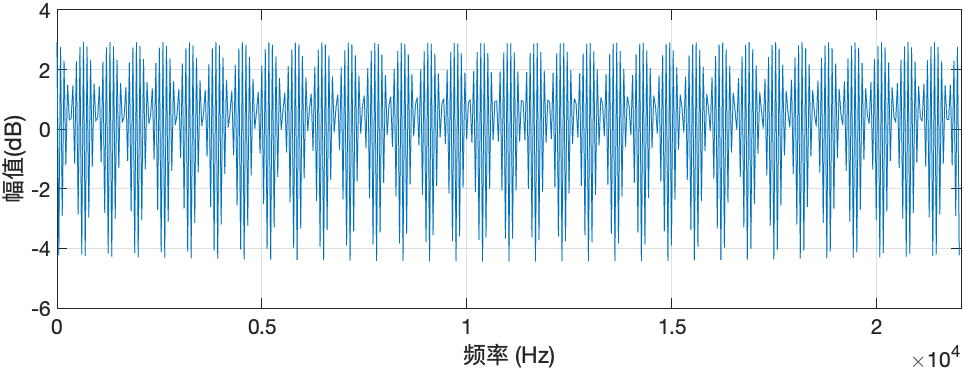
\includegraphics[width=2in]{Image/FIRCombResponse.png}
    }
    \subfigure[IIR comb filter]{
	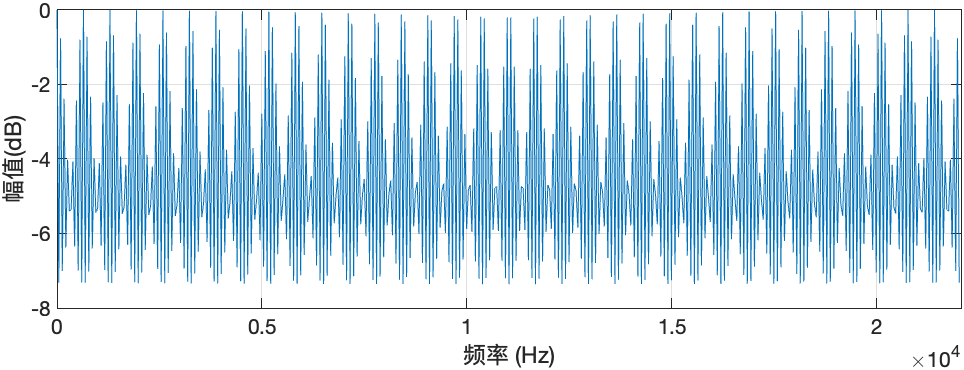
\includegraphics[width=2in]{Image/IIRCombResponse.png}
    }
    \\
    \subfigure[Universal comb filter]{
    	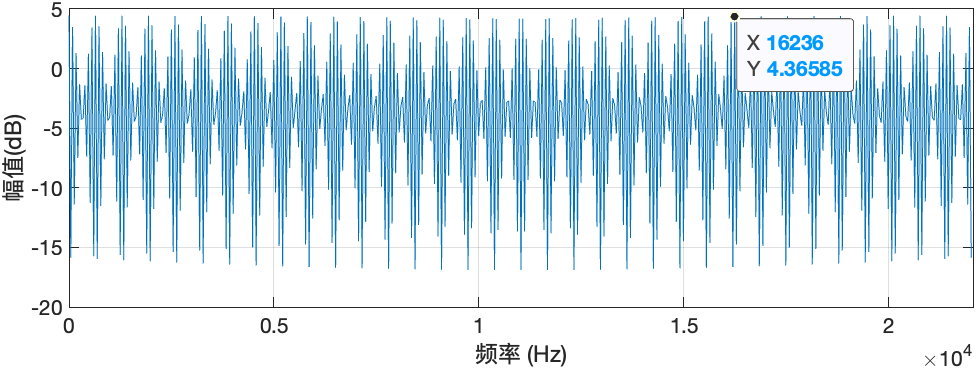
\includegraphics[width=2in]{Image/UniversalCombResponse.png}
    }
    \subfigure[Natural comb filter]{
    	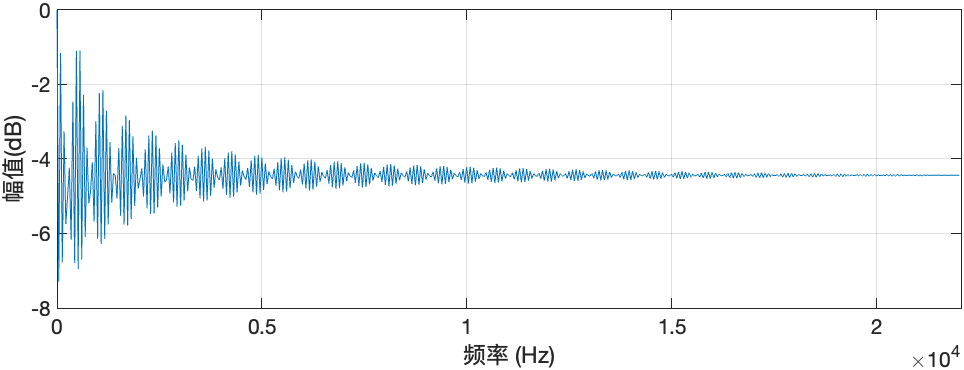
\includegraphics[width=2in]{Image/NaturalCombResponse.png}
    }
    \caption{Frequency response of different structure filters}
\end{figure}
From Figure 10, it can be seen that the response of FIR comb filter and IIR comb filter are symmetric about the transverse axis. The universal comb filter is the combination of them, whose frequency response contains both characteristics of FIR and IIR comb filter. Natural comb filter has the response consistent with IIR comb filter before the cut-off frequency of its low-pass filter. Then I use them to filter a same audio signal separately and give an evaluation in Table 4.
\begin{table}[ht]
	\centering
	\fontfamily{ppl}\selectfont
	\begin{tabular}{l l l l l}
		\toprule
		 & distortion & visibility & humidity & fullness \\
		\midrule
		FIR comb filter & 3 & 4 & 4 & 4 \\
		IIR comb filter & 4 & 4 & 3 & 3 \\
		Universal comb filter & 3 & 5 & 4 & 4 \\
		Natural comb filter & 5 & 4 & 3 & 2 \\
		\bottomrule
	\end{tabular}
	\caption{Evaluation of basic comb filters}
	\label{tab:normaltab}
	\setfloatalignment{b} % Position the table caption at the bottom of the table
\end{table}

Here I evaluate the comb filters in four dimensions, as distortion, visibility, humidity and fullness. 'Distortion' reflects the distortion level of the audio signal being filtered, 'visibility' means the significance of delay effect under the same delay time parameter setting. 'Humidity' and 'fullness' are often used in subjective evaluation of sound quality, which reflect the auditory quality of sound. From the evaluation results, it can be seen that the universal comb filter has the most significant delay effect. When I listened to the processing result of universal comb filter, I could even hear delayed sound effects more than twice, which is actually due to its structure. Natural comb filter provides the delay effect with minimal distortion but also reducing the fullness of sound because of the low-pass filter in it. FIR and IIR comb filter are similar, FIR comb filter has stronger sound expression and IIR comb filter has better sound effects.

Then, I evaluate the improved comb filters in the same way. There are three different structures and their response are shown as Figure 11.
\begin{figure}[h!]
    \centering
    \subfigure[FIR direct path improved]{
        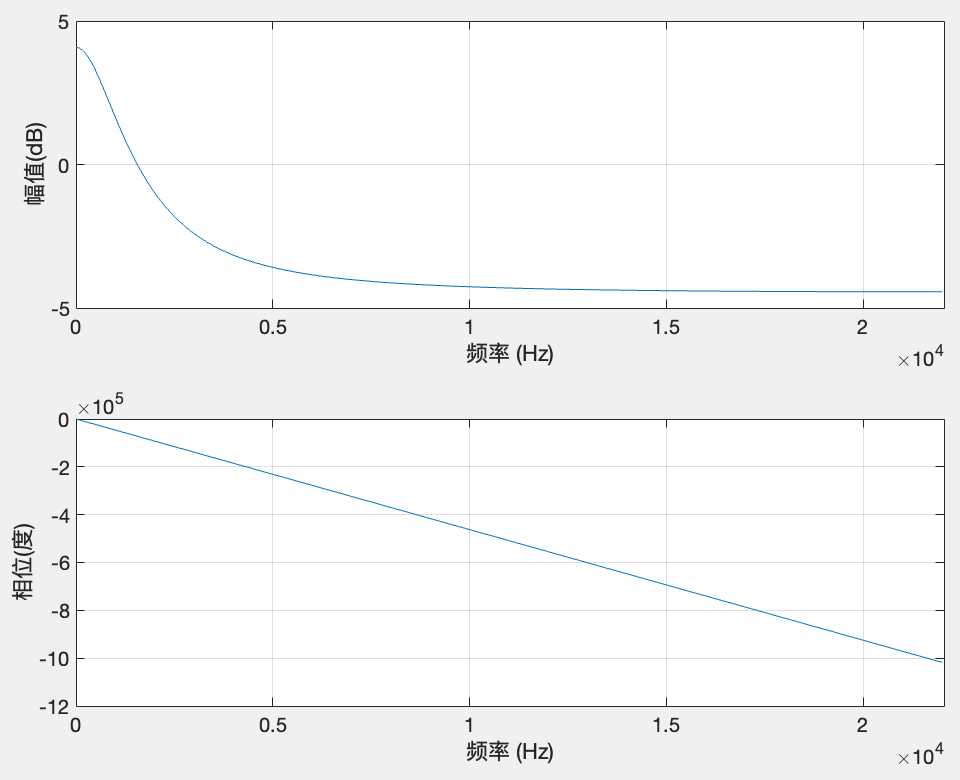
\includegraphics[width=2in]{Image/FIRDirect.png}
    }
    \subfigure[FIR side path improved]{
	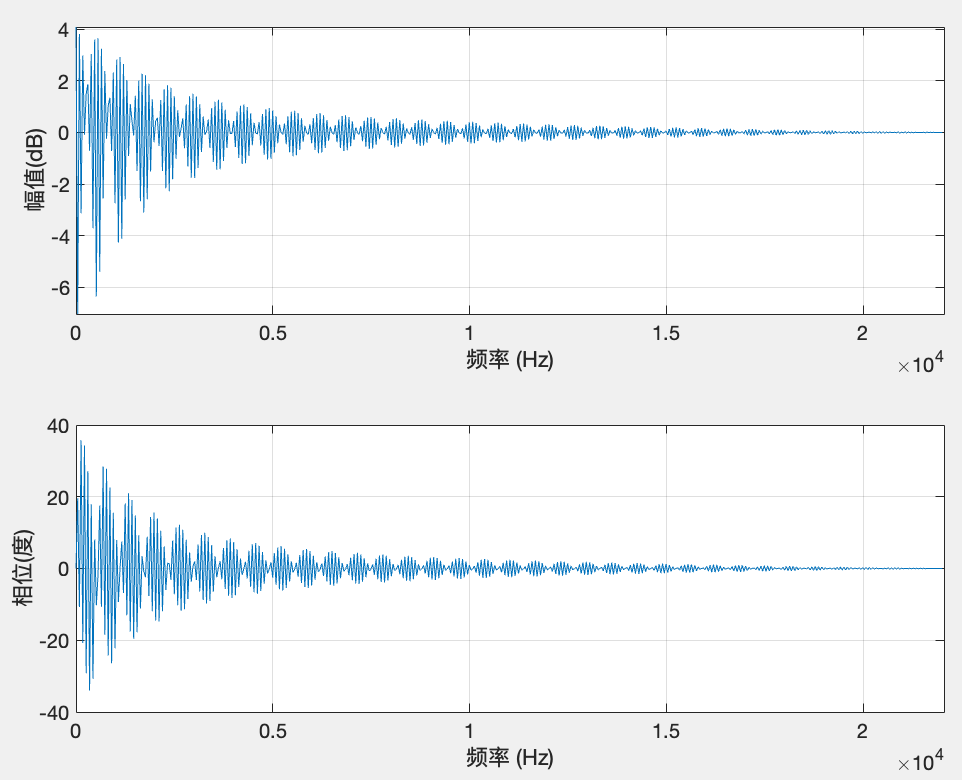
\includegraphics[width=2in]{Image/FIRReflected.png}
    }
    \subfigure[Universal comb improved]{
    	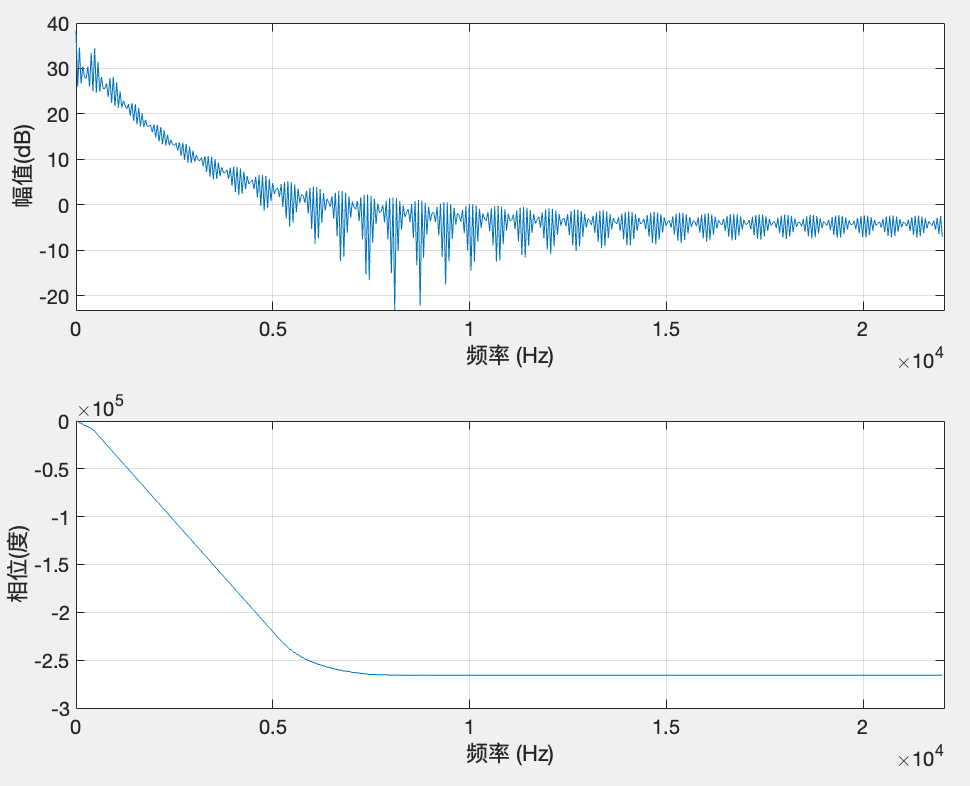
\includegraphics[width=2in]{Image/NaturalUniversal.png}
    }
    \caption{Frequency and phase response of improved filters}
\end{figure}
If we add low-pass filter to the direct path, the FIR filter will still be linear phase. But if we add it to the side-chain, the filter will become no more linear phase. The frequency response of improved structure as Figure 9 looks like the combination of the two above when its phase response is also approximately linear. 
\begin{table}[ht]
	\centering
	\fontfamily{ppl}\selectfont
	\begin{tabular}{l l l l l}
		\toprule
		 & distortion & visibility & humidity & fullness \\
		\midrule
		Direct path & 2 & 1 & 3 & 3 \\
		Side path & 5 & 5 & 3 & 4 \\
		Universal & 1 & 5 & 2 & 3 \\
		\bottomrule
	\end{tabular}
	\caption{Evaluation of improved comb filters}
	\label{tab:normaltab}
	\setfloatalignment{b} % Position the table caption at the bottom of the table
\end{table}

Adding low-pass filters to all paths of universal comb filter will cause extremely severe distortion to the sound. Even if I have  set BL, FF and FB to extremely small values, there is no improvement in the situation either. Maybe I have a wrong formula derivation for it or some other problems. Whatever, adding low-pass filter to the direct path of FIR comb filter may cause the disappearance of direct sound and the delay effect will not be reflected either. So adding low-pass filter to side path looks like the best choice, which won't attenuate direct sound, ensuring significant delay effects while also preventing distortion of the sound.

\section{DISCUSSION AND CONCLUSION}
In this report, I implement seven different structures of comb filters, then I make subjective and objective evaluation on them. Wherein universal comb filter has the best result but the improved structure of universal comb filter exists extremely serious distortion. For a further research, the transform function of improved universal comb filter still needs improvement. Besides, other types of filters, such as band-pass or peak filter, can also be added into the comb filter to form new sound effects.

\end{document}